\documentclass[a4paper]{article}

\usepackage[utf8]{inputenc}
\usepackage[danish]{babel}
\usepackage [T1]{fontenc}
\usepackage{graphicx}
\usepackage{hyperref}
\usepackage{listings}
\lstset{basicstyle=\footnotesize\ttfamily,breaklines=true}

\title{Introduktion til terminalen i Windows, Osx, og Linux}
\author{Hans Jacob T. Stephensen og Jon Sporring }

\begin{document}
\maketitle

\section{Terminalen}

Som borger i det digitale samfund vi i dag vant til den pæne brugerflade som nutidens populære styresystemer forsyner os med. Som datalog vil man ofte få brug for at tilgå nogle af computerens funktionaliteter som besværliggøres af netop denne brugerflade. Terminalen, som også kaldes kommandolinjen i Windows, er datalogen højre hånd. Terminalen er et simpelt program, som har til formål at tilvejebringe brugeren ønsker i form af tekst-kommandoer. Næsten alle de opgaver, der kan laves med den grafiske brugerflade kan laves i terminalen og omvendt. Vi vil først og fremmest drage nytte af den terminalens direkte kontrol over de programmer, vi skriver, og videre i din uddannelse vil du have gavn af den hurtige og rå information, som man får igennem terminalen.

\section{Den hierarkiske mappestruktur}

Når du åbner en mappe i dit foretrukne styresystem vil mappen have en placering i det aktive filsystem, hvad enten det er fra terminalen eller via operativsystemets grafiske brugergrænseflade. Terminalen vil stort set altid være tilknyttet en bestemt mappe i filsystemet, og man siger at det er den mappe som terminalen "`står"' i. Den præcise struktur som filsystemer har, varierer imellem Linux, MaxOS X og Windows, men fælles er den hierarkiske opbygning. Dette er illustreret i Figure~\ref{fig:filhierakier}.
\begin{figure}
  \begin{center}
    % \scalebox{0.23}
    {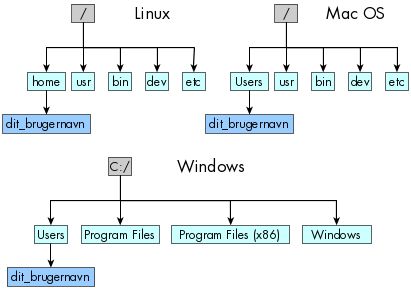
\includegraphics[width=\textwidth]{filehira.png}}
  \end{center}
  \caption{Toppen af filhierarkier i forskellige operativsystemer.}
  \label{fig:filhierakier}
\end{figure}
 Når du begynder at arbejde i terminalen på din nuværende computer er det praktisk både at forestille sig strukturen du kender med mapper og filer i mapper, samt den hierarkiske struktur.

\section{De vigtigste kommandoer}
Der findes et væld af terminalkommandoer, man kan køre fra terminalen, og man kan selv lave yderligere. I det følgende vil vi gennemgå de kommandoer, som er vist i Tabel~\ref{tab:kommandoer}, i de 3 forskellige operativsystemer.
\begin{table}
  \centering
  \begin{tabular}{|l||p{0.5\linewidth}|}
    \hline
    Kommando & Beskrivelse 
    \\ \hline\hline
    \begin{tabular}[t]{ll}
      Windows: &\texttt{dir}
      \\OSX: &    \texttt{ls} 
      \\Linux: & \texttt{ls}   
    \end{tabular}
              & Vis nuværende mappes indhold. 
    \\ \hline
    \begin{tabular}[t]{ll}
      Windows: &\texttt{cd <mappe>} 
      \\OSX: &    \texttt{cd <mappe>} 
      \\Linux: & \texttt{cd <mappe>} 
    \end{tabular}
              & få terminalen til at pege på \texttt{<mappe>} i stedet for den nuværende mappe. 
    \\ \hline
              % \texttt{touch <fil>} & opret en tom fil med navnet \texttt{<fil>}. \\ \hline
    \begin{tabular}[t]{ll}
      Windows: &\texttt{emacs <fil>}
      \\OSX: &    \texttt{emacs <fil>}\\ & \texttt{open -a aquamacs <fil>}
      \\Linux: & \texttt{emacs <fil>} 
    \end{tabular}
               & Åben \texttt{<fil>} i emacs hvis den findes i den nuværende mappe. Findes den ikke oprettes den her automatisk. 
    \\ \hline
    \begin{tabular}[t]{ll}
      Windows: &\texttt{mkdir <mappe>}
      \\OSX: &    \texttt{mkdir <mappe>} 
      \\Linux: & \texttt{mkdir <mappe>}   
    \end{tabular}
                 & opret \texttt{<mappe>}. \\ \hline
    \begin{tabular}[t]{ll}
      Windows: &\texttt{rmdir <mappe>}
      \\OSX: &    \texttt{rmdir <mappe>}
      \\Linux: & \texttt{rmdir <mappe>}
    \end{tabular}
               & slet \texttt{<mappe>}. \\ \hline
    \begin{tabular}[t]{ll}
      Windows: &\texttt{move <fil> <mappe>}
      \\OSX: &    \texttt{mv <fil> <mappe>}
      \\Linux: & \texttt{mv <fil> <mappe>}
    \end{tabular}
               & Flyt \texttt{<fil>} ind i \texttt{<mappe>}. \\ \hline
    \begin{tabular}[t]{ll}
      Windows: &\texttt{copy <fil> <mappe>}
      \\OSX: &    \texttt{cp <fil> <mappe>}
      \\Linux: & \texttt{cp <fil> <mappe>}
    \end{tabular}
               & Kopier \texttt{<fil>} ind i \texttt{<mappe>}. \\ \hline
    \begin{tabular}[t]{ll}
      Windows: &\texttt{del <fil>}
      \\OSX: &    \texttt{rm <fil>}
      \\Linux: & \texttt{rm <fil>}
    \end{tabular}
               & slet \texttt{<fil>} (Advarsel: Dette kan ikke fortrydes). \\ \hline
    \begin{tabular}[t]{ll}
      Windows: &\texttt{echo <streng | variabel>}
      \\OSX: &    \texttt{echo <streng | variabel>}
      \\Linux: & \texttt{echo <streng | variabel>}
    \end{tabular}
               & skriv en streng eller indholdet af en variabel til skærmen. \\ \hline
  \end{tabular}\\
  \caption{Tabel over de vigtigeste kommandoer i terminalen}
  \label{tab:kommandoer}
\end{table}

\subsection{Windows.}

Windows 7 og tidligere: Du åbner terminalen ved at trykke på \textit{Start->Run} i nederste venstre hjørne, og derefter skrive \texttt{cmd} i boksen. Nu skal der gerne åbnes et terminal vindue med en prompt der viser noget ala
\begin{lstlisting}[frame=single]
Microsoft Windows [Version 6.1.7601]
Copyright <c> 2009 Microsoft Corporation.  All rights reserved.

C:\Users\sporring>
\end{lstlisting}
Hvis du vil se, hvilke filer, som ligger i mappen skriver du
\begin{lstlisting}[frame=single]
C:\> dir
 Volume in drive C has no label.
 Volume Serial Number is 94F0-31BD

 Directory of C:\Users\sporring

30-07-2015  14:27    <DIR>       .
30-07-2015  14:27    <DIR>       ..
30-07-2015  14:27    <DIR>       Contacts
30-07-2015  14:27    <DIR>       Desktop
30-07-2015  14:27    <DIR>       Documents
...
30-07-2015  14:27    <DIR>       Videos
                           0 File(s)                 0 bytes
                          13 Dir(s)  96.825.036.800 bytes free
\end{lstlisting}
hvoraf man kan se, at der er ingen filer og 13 mapper (DIR), dato og tid for deres oprettelse i de 2 venstre kolonner, deres størrelse eller om det er en mappen, samt deres navne i højre kolonne.

Hvis du vil skifte mappe til \texttt{Documents} skriver du
\begin{lstlisting}[frame=single]
C:\> cd Documents

C:\Users\dirsporring\Documents>
\end{lstlisting}
som er den samme mappe, som Windows Explorer finder, når man trykker på \texttt{Dokumenter}. På en ny computer er denne mappe typisk tom,
\begin{lstlisting}[frame=single]
C:\> dir
 Volume in drive C has no label.
 Volume Serial Number is 94F0-31BD

 Directory of C:\Users\sporring\Documents

30-07-2015  14:27    <DIR>       .
30-07-2015  14:27    <DIR>       ..
                           0 File(s)                 0 bytes
                           2 Dir(s)  96.825.036.800 bytes free
\end{lstlisting}
Hvis du vil oprette en ny mappe f.eks.\ med navn \texttt{fsharp}, der hvor du står, skriver du
\begin{lstlisting}[frame=single]
C:\Users\dirsporring\Documents> mkdir fsharp

C:\Users\dirsporring\Documents>
\end{lstlisting}
Og du kan sikre dig, at den er oprettet ved igen at bruge \texttt{dir} kommandoen,
\begin{lstlisting}[frame=single]
C:\> dir
 Volume in drive C has no label.
 Volume Serial Number is 94F0-31BD

 Directory of C:\Users\sporring\Documents

30-07-2015  14:27    <DIR>       .
30-07-2015  14:27    <DIR>       ..
30-07-2015  14:27    <DIR>       fsharp
                           0 File(s)                 0 bytes
                           3 Dir(s)  96.825.036.800 bytes free
\end{lstlisting}

noget med echo, path, hvordan path sættes, piping og move, rmove...

\subsection{Linux.}

Du åbner en terminal ved at taste\footnote{Andre Linux distributioner kan have anden tast kombination. f.eks. \texttt{Super + T}.} \texttt{Ctrl + Alt + T}. Du bør nu kunne se en terminal med en linje som angiver dit brugernavn, computernavn og terminalens nuværende placering i filsystemet. Tegnet $\sim$ bruges i Linux til at angive din egen Home-mappe. Trykker du \texttt{Enter}, vil terminalen udfører en kommando uden indhold, afslutte den nuværende linje og give dig en ny. En blinkende markør vil angive den aktive linje. De vigtigste kommandoer du vil få brug for er

Hvis du i din Home-mappe opretter en mappe \texttt{studie} med en undermappe \texttt{pop}, igen med undermapper \texttt{noter} og \texttt{uge1}, samt en fil med navnet \texttt{terminalNoter.txt}, så kan din terminal f.eks. se således ud:

\begin{lstlisting}[frame=single, language=bash]
bruger@computer:~$ mkdir studie
bruger@computer:~$ cd studie/
bruger@computer:~/studie$ mkdir pop
bruger@computer:~/studie$ cd pop/
bruger@computer:~/studie/pop$ mkdir uge1
bruger@computer:~/studie/pop$ mkdir noter
bruger@computer:~/studie/pop$ ls noter  terminalNoter.txt  uge1
bruger@computer:~/studie/pop$ mv terminalNoter.txt noter/
bruger@computer:~/studie/pop$
\end{lstlisting}
Ønsker du derpå at skrive i documented \texttt{terminalNoter.txt} kan du directe fra din home mappe skrive
\begin{verbatim}
bruger@computer:~$ emacs studie/pop/noter/terminalNoter.txt
\end{verbatim}
eller alternativt få terminalen til først at pege på mappen \texttt{noter} og derpå åbne documentet ved
\begin{verbatim}
bruger@computer:~$ cd studie/pop/noter/
bruger@computer:~/studie/pop/noter$ emacs terminalNoter.txt
\end{verbatim}

I Linux har man muligheden for at få terminalen til at gætte på hvad man er ved at skrive ved at trykke \texttt{tab}, hvorpå resten af kommandoen ofte vil blive automatisk færdiggjort. Desuden kan manualer til de fleste kommandoer kan findes ved at skrive \texttt{man} foran kommandoen. Manualen til \texttt{rm} kan f.eks. fås ved at skrive \texttt{man rm}. Ønsker du at afbryde terminalen i dens arbejde kan dette ofte gøres ved at trykke \texttt{Ctrl+Z}.

\subsection{MacOS X.}

[OBS: MANGLER]

% \section{Compilering af \texttt{F\#} programmer}

% \subsection{Linux.}

% Hvis \texttt{F\#} er succesfuld installeret på din maskine, kan du i terminalen skrive \texttt{fsharpi}.
% Pg har du skrevet et program i en kildekode fil med navnet \texttt{mitprogram.fsx} kan du oversætte det til maskinkode ved at i terminalen at skrive \texttt{fsharpc mitprogram.fsx} - hvortil en ny eksekverbar fil med navnet \texttt{mitprogram.exe} vil blive skrevet til samme mappe. Hvis compileringen er en succes vil din terminal have følgende stående:

% \begin{verbatim}
% bruger@computer:~$ fsharpc mitprogram.fsx
% F# Compiler for F# 3.1 (Open Source Edition)
% Freely distributed under the Apache 2.0 Open Source License
% bruger@computer:~$
% \end{verbatim}

% \subsection{MacOS X.}

% [OBS: MANGLER]

% \subsection{Windows.}

% [OBS: MANGLER]


\end{document}